\documentclass[conference]{IEEEtran}

\usepackage[brazilian]{babel}
\usepackage[utf8]{inputenc}
\usepackage[T1]{fontenc}
\usepackage{graphicx}
\usepackage{float}      
\usepackage{amsmath,amssymb}
\usepackage{siunitx}
\usepackage{booktabs}
\usepackage{cite}
\usepackage[caption=false,font=footnotesize]{subfig} 
\graphicspath{{figures/}} 
\usepackage[hidelinks]{hyperref}

\sisetup{per-mode=symbol,detect-all}
\title{\textbf{Transferência de Energia Sem Fio}\\\large Compensação série-série}
\author{\IEEEauthorblockN{José Vítor Cardozo Amaral}
\IEEEauthorblockA{Universidade Federal de Mato Grosso do Sul\\
Email: vitor.cardozo@ufms.br}
}

\begin{document}
\maketitle
\begin{abstract}
 Este trabalho apresenta o projeto e a validação, em \emph{MATLAB/Simulink}, de um sistema de Transferência de Energia sem Fio com compensação série–série (SS) para \SI{500}{\watt} em \SI{50}{\kilo\hertz}, considerando $k{=}0{,}4$, $V_s{=}\SI{400}{\volt}$ (RMS) e $R_c{=}\SI{320}{\ohm}$. A metodologia realiza varreduras em $L_p$ e $L_s$.  As simulações temporais confirmaram fator de potência praticamente unitário e alto rendimento. Observou-se que a eficiência na região selecionada depende predominantemente de $L_s$, enquanto a janela de $|V_p|$ delimita o conjunto de soluções viáveis. Os resultados corroboram a viabilidade do arranjo SS para a potência-alvo, oferecendo um fluxo de dimensionamento objetivo e reproduzível.
\end{abstract}
\begin{IEEEkeywords}
Transferência de Energia sem fio; acoplamento Indutivo; série–série; ressonância; MATLAB; Simulink.
\end{IEEEkeywords}

\section{Introdução}
A Transferência de Energia/Potência sem Fio por acoplamento indutivo tem ampla aplicação, de eletrônicos de consumo e dispositivos biomédicos à mobilidade elétrica e robótica, por eliminar conectores, operar em ambientes agressivos e permitir acoplamento em movimento. O princípio baseia-se em bobinas magneticamente acopladas, sendo uma primária, geradora de campo magnético, e outra secundária, onde haverá tensão ou corrente induzida a partir das linhas de campo primárias \cite{godoy2024wpt}.
Entre as topologias clássicas de compensação, a \textbf{série–série (SS)} apresenta peculiaridades relevantes para o projeto. Quando corretamente \emph{compensada}, a rede SS \emph{não} reflete a parcela imaginária ao primário e o \textbf{dimensionamento do capacitor primário \(C_p\) não depende da indutância mútua \(M\)}; com isso, a sintonia do lado primário torna-se simples e o ponto de compensação não é deslocado por variações do acoplamento \cite{godoy2024wpt}. Em contrapartida, \textbf{reduções do acoplamento} e \textbf{desintonias modestas} podem levar o sistema à \emph{instabilidade associada à bifurcação}: a potência transferida pode escalar para valores muito acima do nominal projetado enquanto a eficiência se degrada. Por outro lado, \emph{evitar} a região de bifurcação traz uma operação SS \textbf{muito estável}, desde que a rede seja projetada para a vizinhança de ressonância pretendida. Esses compromissos tornam a SS atraente pela simplicidade e previsibilidade próximas à ressonância, mas exigem critérios de seleção que respeitem limites de tensão/corrente e fator de potência.
\textbf{Aplicação e organização do artigo}: Este trabalho aplica um fluxo de projeto em \emph{MATLAB/Simulink} para uma compensação SS visando \SI{500}{\watt} a partir de uma tensão de saída de \SI{400}{\volt}, em \SI{50}{\kilo\hertz}, com acoplamento nominal $k{=}0{,}4$. Apresentamos: (i) equações do modelo; (ii) varredura em \(L_p\) e \(L_s\) com critérios de seleção (incluindo uma janela em $|V_p|$); e (iii) análise em \emph{Simulink} para simulação e validação do projeto. O artigo está organizado como segue: Seção~II descreve a visão geral do sistema e a metodologia; Seção~III traz resultados (mapas/gráficos); Seção~IV apresenta a análise detalhada no \emph{Simulink}; e a Seção~V conclui.
\section{Visão Geral do Sistema e Metodologia}
\subsection{Arquitetura do sistema (SS)}
O sistema adota compensação série–série (SS): uma fonte AC alimenta $L_p$–$C_p$ (primário), acoplado magneticamente com $L_s$–$C_s$ (secundário) por meio da indutância mútua $M$. A resistência da carga é representada por $R_c$ e as resistências da bobina primária e secundária por $R_p$ e $R_s$, respectivamente.
\begin{figure}[H]
  \centering
  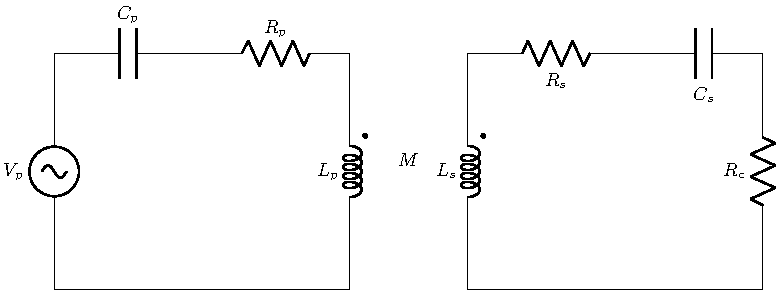
\includegraphics[width=\linewidth]{topo.pdf}
  \caption{Topologia série–série (SS) do sistema.}
  \label{fig:topo-ss}
\end{figure}

\subsection{Metodologia do projeto (do script de varredura ao caso de simulação)}
O procedimento automatiza a seleção de $L_p$ e $L_s$ via varreduras 2D e critérios de viabilidade/seleção, seguido de validação no \emph{Simulink}:
\textbf{(1) Alvos e constantes do projeto.}
Define-se $V_s$, $R_c$, $f$ ($\omega_0{=}2\pi f$), $k$ (acoplamento) e a faixa permitida de $V_p$. A corrente e a potência de saída especificadas no projeto são
\begin{equation}\label{eq:iout}
I_{out} = \frac{V_s}{R_c},
\end{equation}
\begin{equation}\label{eq:pout}
P_{out} = R_c\,|I_{out}|^2 \;=\; \frac{V_s^2}{R_c}.
\end{equation}
fixando o requisito de \SI{500}{\watt} quando $V_s{=}\SI{400}{\volt}$ e $R_c{=}\SI{320}{\ohm}$.
\textbf{(2) Varreduras.}
Varrer $L_p$ e $L_s$ em malha regular (passo $10~\mu$H), formando as grades $LP$ e $LS$.
\textbf{(3) Perdas concentradas.}
Modelar resistências série proporcionais à indutância:
\[
 R_p=\alpha L_p,\quad R_s=\alpha L_s,\quad \alpha=1000~\Omega/\text{H},
\]
gerando as malhas $RP$ e $RS$.
\textbf{(4) Capacitores série.}
Obtêm-se as malhas $CP$ e $CS$:
\begin{equation}\label{eq:CpCs}
C_p = \frac{1}{L_p\,\omega_0^2},\qquad
C_s = \frac{1}{L_s\,\omega_0^2}.
\end{equation}

\textbf{(5) Acoplamento e impedâncias.}
O acoplamento magnético é
\begin{equation}\label{eq:M_again}
M = k\,\sqrt{L_p L_s}.
\end{equation} Impedância no secundário:
\begin{equation}
\label{eq:Zs_total}
Z_s(j\omega_0)=R_s+j\omega_0 L_s+\frac{1}{j\omega_0 C_s}+R_c.
\end{equation}
A impedância refletida ao primário e a impedância do primário são, respectivamente:
\begin{align}
\label{eq:Zr}
Z_{\text{r}}(j\omega_0)&=\frac{(j\omega_0 M)^2}{Z_s(j\omega_0)},\\
\label{eq:Zp}
Z_p(j\omega_0)&=R_p+j\omega_0 L_p+\frac{1}{j\omega_0 C_p},
\end{align}
e a impedância total no primário é
\begin{equation}
\label{eq:Ztot}
Z(j\omega_0)=Z_p(j\omega_0)+Z_{\text{r}}(j\omega_0).
\end{equation}
\textbf{(6) Variáveis.}
Corrente de entrada e tensão no primário:
\begin{equation}
\label{eq:IinVp}
I_{in}=\frac{I_{out}\,Z_s(j\omega_0)}{j\omega_0 M},\qquad V_p=Z(j\omega_0)\,I_{in},
\end{equation}
de onde se obtêm $S_{in}=V_p I_{in}^*$, $P_{in}=\Re\{S_{in}\}$, $Q_{in}=\Im\{S_{in}\}$ e a eficiência
\begin{equation}
\label{eq:eta}
\eta=\frac{P_{out}}{P_{in}}.
\end{equation}
\textbf{(7) Critério de seleção.}
Aplica-se uma janela sobre o módulo da tensão no primário:
\[
|V_p|\in[V_{\min},V_{\max}],\quad V_{\min}=\SI{350}{V},\; V_{\max}=\SI{400}{V},
\]
retendo os pares $(L_p,L_s)$ que satisfazem simultaneamente as condições. 
\textbf{(8) Caso selecionado e validação no \emph{Simulink}.}
O par selecionado $(L_p,L_s)$ e seus correspondentes $(R_p,R_s,C_p,C_s)$ são então levados ao \emph{Simulink} para validação.
Os resultados de simulação são discutidos na Seção~IV.
\subsection{Dados de projeto}
Os parâmetros utilizados nas varreduras e na seleção são sumarizados na Tabela~\ref{tab:dados}.
\begin{table}[H]
  \caption{Dados de Projeto (varreduras e seleção)}
  \label{tab:dados}
  \centering
  \begin{tabular}{lll}
    \toprule
    Parâmetro & Símbolo & Valor \\
    \midrule
    Tensão de especificação & $V_s$ & \SI{400}{V} \\
    Carga & $R_c$ & \SI{320}{\ohm} \\
    Frequência & $f$ & \SI{50}{kHz} \\
    Acoplamento nominal & $k$ & $0{,}4$ \\
    Potência-alvo & $P_{out}$ & \SI{500}{\watt} \\
    Faixa de $|V_p|$ & $|V_p|$ & \SI{350}{}–\SI{400}{\volt} \\
    \bottomrule
  \end{tabular}
\end{table}

\section{Resultados}

\subsection{Gráficos de seleção}
A Fig.~\ref{fig:fig1} reúne os quatro painéis gerados no MATLAB a partir da varredura $L_p\times L_s$:
\begin{itemize}
  \item \textbf{(a)} Mapa de $|V_p|$ (superfície) no plano $(L_p,L_s)$.
  \item \textbf{(b)} Nuvem de \emph{pontos válidos} que satisfazem a janela $|V_p|\in[\SI{350}{\volt},\SI{400}{\volt}]$.
  \item \textbf{(c)} Mapa de eficiência $\eta$ (superfície) no plano $(L_p,L_s)$.
  \item \textbf{(d)} \emph{Corte 1D} de $\eta$ em função de $L_s$ (mantendo $L_p=\SI{2211}{\micro\henry}$). Nesta região, a eficiência depende \emph{predominantemente} de $L_s$, de modo que (d) é essencialmente o “perfil” do mapa (c) ao longo do eixo $L_s$.
\end{itemize}

\begin{figure*}[!t]
  \centering
  \subfloat[]{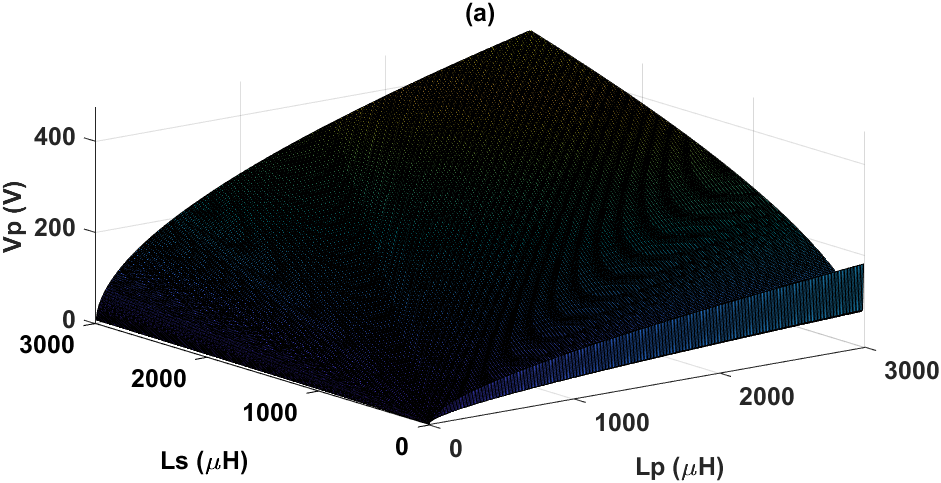
\includegraphics[width=0.48\linewidth]{a.png}\label{fig1:a}}\hfill
  \subfloat[]{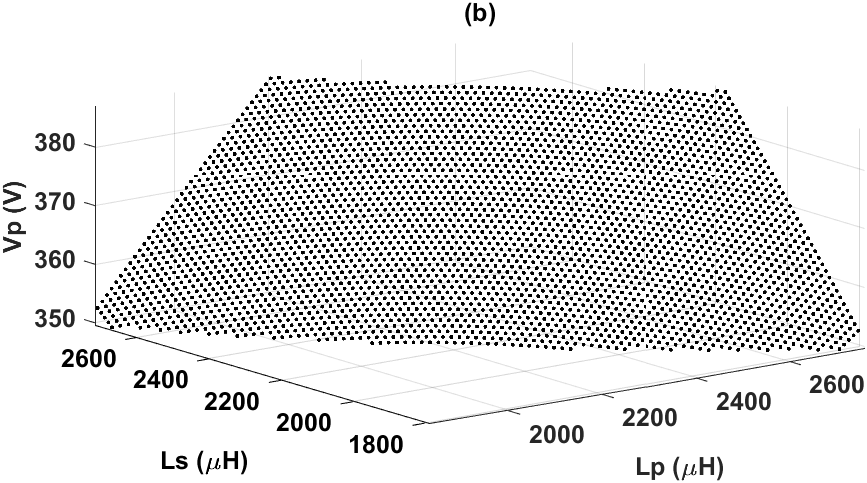
\includegraphics[width=0.48\linewidth]{b.png}\label{fig1:b}}\\[1ex]
  \subfloat[]{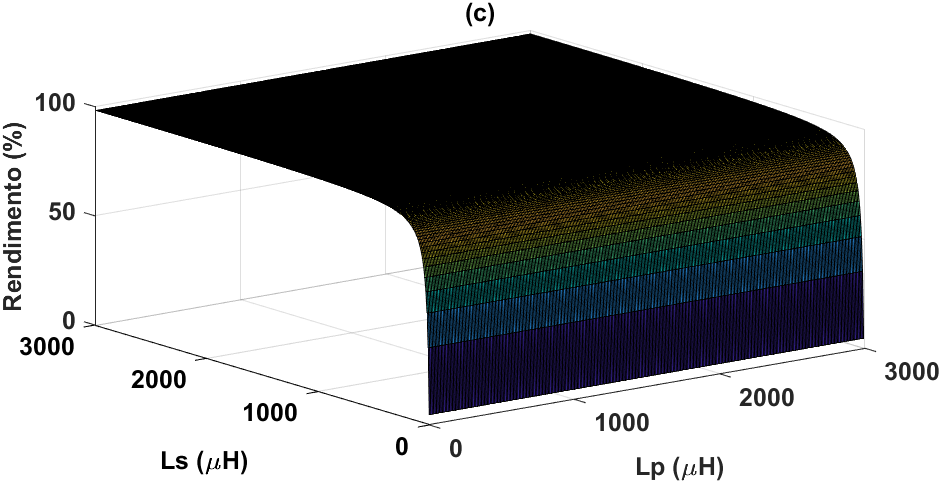
\includegraphics[width=0.48\linewidth]{c.png}\label{fig1:c}}\hfill
  \subfloat[]{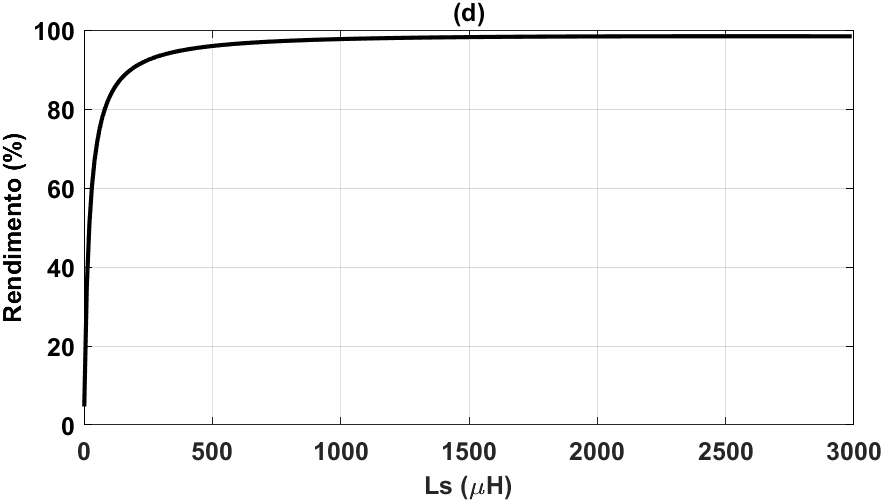
\includegraphics[width=0.48\linewidth]{d.png}\label{fig1:d}}
  \caption{Resultados da varredura e seleção: (a) mapa de $|V_p|$; (b) pontos que atendem $|V_p|\in[\SI{350}{\volt},\SI{400}{\volt}]$; (c) mapa de eficiência $\eta$; (d) corte $\eta(L_s)$}
  \label{fig:fig1}
\end{figure*}

Devido às exigências do projeto, foi necessário aumentar a faixa das indutâncias para valores acima de \SI{2}{\milli\henry}.\\
Para destacar a região útil da seleção, a Fig.~\ref{fig:pontos} mostra um \emph{zoom} do painel (b), evidenciando a concentração de soluções ao redor do par escolhido, juntamente com os valores de $L_p$ e $L_s$ selecionados.
\begin{figure}[t]
  \centering
  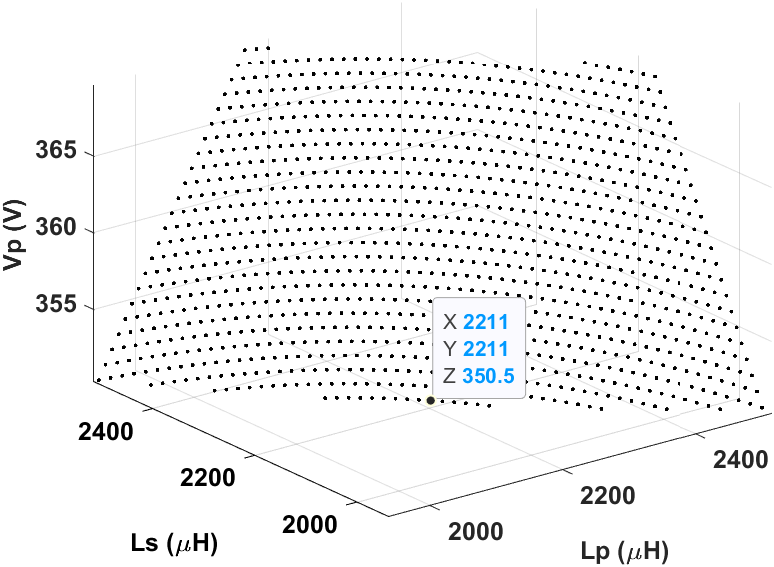
\includegraphics[width=\linewidth]{selecao.png}
  \caption{\emph{Zoom} dos pontos válidos (janela de $|V_p|$) e seleção das indutâncias.}
  \label{fig:pontos}
\end{figure}

\subsection{Variáveis calculadas}
Com base no par selecionado $(L_p,L_s)=(\SI{2,211}{\milli\henry})$, $k=\num{0.4}$, $f=\SI{50}{\kilo\hertz}$, $R_c=\SI{320}{\ohm}$ e $V_s=\SI{400}{\volt}$ (RMS), obtêm-se:
\begin{itemize}
  \item \textbf{Capacitores série}: $C_p=C_s=\dfrac{1}{L\,\omega_0^2}$ com $\omega_0=2\pi f \Rightarrow C_p=C_s\approx \SI{4.583}{\nano\farad}$.
  \item \textbf{Perdas concentradas}: $R_p=1000\,L_p$ e $R_s=1000\,L_s \Rightarrow R_p=R_s\approx \SI{2.211}{\ohm}$.
  \item \textbf{Acoplamento}: $M=k\sqrt{L_pL_s}\Rightarrow M\approx \SI{884.4}{\micro\henry}$.
  \item \textbf{Grandezas de especificação}: $I_{out}=V_s/R_c=\SI{1.25}{\ampere}$ (RMS) e $P_{out}=V_s^2/R_c=\SI{500}{\watt}$.
  \item \textbf{Ponto selecionado (janela)}: módulo da tensão no primário dentro da janela, com $|V_p|=\SI{350.50}{\volt}$ (RMS).
\end{itemize}

\subsection{Tabela com dados calculados}
A Tabela~\ref{tab:dados_calc_nominal} resume os \textbf{dados calculados do caso selecionado} (nominal, \SI{50}{\kilo\hertz}), \emph{sem} listar impedâncias.
\begin{table}[H]
  \caption{Dados calculados (nominal, $f=\SI{50}{\kilo\hertz}$)}
  \label{tab:dados_calc_nominal}
  \centering
  \begin{tabular}{lcc}
    \toprule
    Quantidade & Símbolo & Valor \\
    \midrule
    Tensão de saída & $V_s$ & \SI{400}{\volt} \\
    Carga equivalente & $R_c$ & \SI{320}{\ohm} \\
    Frequência & $f$ & \SI{50}{\kilo\hertz} \\
    Fator de acoplamento & $k$ & \num{0.4} \\
    Indutâncias & $L_p, L_s$ & $\SI{2211}{\micro\henry}$ \\
    Resistências série & $R_p, R_s$ & $\SI{2.211}{\ohm}$ \\
    Capacitâncias (SS) & $C_p, C_s$ & $\SI{4.583}{\nano\farad}$ \\
    Indutância mútua & $M$ & \SI{884.4}{\micro\henry} \\
    Corrente de saída (RMS) & $I_{out}$ & \SI{1.25}{\ampere} \\
    Potência de saída & $P_{out}$ & \SI{500}{\watt} \\
    Tensão no primário (RMS) & $|V_p|$ & \SI{350.50}{\volt} \\
    \bottomrule
  \end{tabular}
\end{table}

\section{Análise de Resultados}
\subsection{Montagem de simulação}
A Fig.~\ref{fig:simc} apresenta a montagem empregada no \emph{Simulink} para análise dos valores obtidos.
\begin{figure}[t]
  \centering
  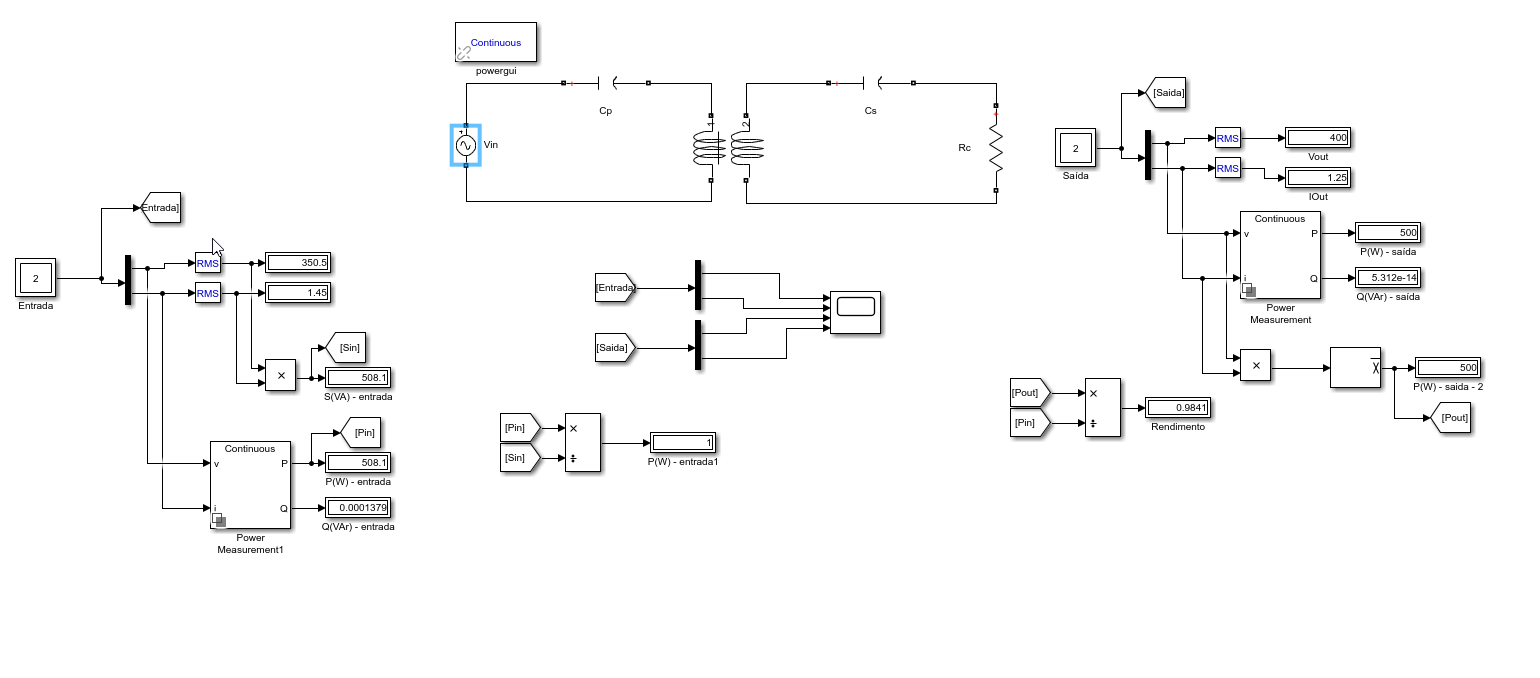
\includegraphics[width=\linewidth]{simc.png}
  \caption{Modelo de simulação no \emph{Simulink}.}
  \label{fig:simc}
\end{figure}
A Tabela~\ref{tab:esforcos_nominal} resume os esforços elétricos principais no ponto nominal (\SI{50}{\kilo\hertz}).
\begin{table}[H]
  \caption{Esforços elétricos (nominal, $f=\SI{50}{\kilo\hertz}$)}
  \label{tab:esforcos_nominal}
  \centering
  \begin{tabular}{lccc}
    \toprule
    Grandeza & Símbolo & RMS & Pico \\
    \midrule
    Tensão no primário & $|V_p|$ & \SI{350.50}{\volt} & \SI{495}{\volt} \\
    Corrente de entrada & $|I_{in}|$ & \SI{1.45}{\ampere} & \SI{2.05}{\ampere} \\
    Corrente no indutor primário & $I_{L_p}$ & \SI{1.48}{\ampere} & \SI{2.10}{\ampere} \\
    Corrente no indutor secundário & $I_{L_s}$ & \SI{1.33}{\ampere} & \SI{1.92}{\ampere} \\
    Tensão no capacitor primário & $V_{C_p}$ & \SI{1028}{\volt} & \SI{1454}{\volt} \\
    Tensão no capacitor secundário & $V_{C_s}$ & \SI{924}{\volt} & \SI{1306}{\volt} \\
    \bottomrule
  \end{tabular}
\end{table}

\subsection{Perdas, potências e fator de potência (nominal)}
A Tabela~\ref{tab:potencias_nominal} apresenta o balanço de potências e o fator de potência no caso nominal (\SI{50}{\kilo\hertz}). As perdas distribuídas correspondem às resistências série $R_p$ e $R_s$.
\begin{table}[H]
  \caption{Balanço de potências e FP (nominal, $f=\SI{50}{\kilo\hertz}$)\footnotesize}
  \label{tab:potencias_nominal}
  \centering
  \begin{tabular}{lcc}
    \toprule
    Quantidade & Símbolo & Valor \\
    \midrule
    Potência de entrada & $P_{in}$ & \SI{508}{\watt} \\
    Potência na carga & $P_{out}$ & \SI{500}{\watt} \\
    Potência reativa & $Q_{in}$ & $0~\mathrm{var}$ \\
    Fator de potência & FP & \num{1} \\
    Rendimento & $\eta=P_{out}/P_{in}$ & \SI{98.41}{\percent} \\
    \bottomrule
  \end{tabular}
\end{table}

\subsection{Variação de frequência (45/50/55 kHz)}
Por fim, apresenta-se a avaliação pedida para a “análise de bifurcação” via variação de frequência em $\{45,50,55\}\,\si{\kilo\hertz}$ \emph{com} $C_p$ e $C_s$ mantidos fixos (sintonizados para \SI{50}{\kilo\hertz}).
\begin{table}[H]
  \caption{Variação de frequência}
  \label{tab:freq_variacao}
  \centering
  \scriptsize
  \setlength{\tabcolsep}{3pt}
  \renewcommand{\arraystretch}{1.15}
  \resizebox{0.98\columnwidth}{!}{%
  \begin{tabular}{
      S[table-format=2.0]
      S[table-format=3.1]
      S[table-format=3.1]
      S[table-format=3.1]
      S[table-format=3.1]
      S[table-format=1.3]
  }
    \toprule
    {$f$} & {$P_{in}$} & {$P_{out}$} & {$Q_{in}$} & {$S_{in}$} & {FP}\\
    {(\si{\kilo\hertz})} & {(\si{\watt})} & {(\si{\watt})} & {(var)} & {(\si{\volt\ampere})} & {(--)} \\
    \midrule
    45 & 626,5 & 613,7 & -282,4 & 687,2 & 0.912 \\
    50 & 508,1 & 500,0 & 0,0 & 508,1 & 1.000 \\
    55 & 483,9 & 476,4 & 59,2 & 487,5 & 0.993 \\
    \bottomrule
  \end{tabular}
  }
\end{table}

Quando a frequência se desvia do valor de projeto, observa-se acréscimo em $|Q_{in}|$ e redução do fator de potência ($FP$), evidenciando maior circulação reativa e deslocamento do ponto de operação, consistente com a operação SS fora da ressonância. Ademais, como a potência transferida após alteração da frequência não extrapolou significativamente o valor projetado, a bifurcação não se mostra crítica para este projeto.
\section{Conclusões}
Este trabalho apresentou o projeto e a validação, em \emph{MATLAB/Simulink}, de um sistema de Transferência de Energia sem Fio com compensação série–série (SS) para \SI{500}{W} em \SI{50}{\kilo\hertz}, considerando $k{=}0{,}4$, $V_s{=}\SI{400}{V}$ (RMS) e $R_c{=}\SI{320}{\ohm}$. A metodologia baseada em varreduras de $L_p$ e $L_s$ com critério de seleção por janela de $|V_p|$ conduziu a uma solução viável e coerente com o comportamento esperado da topologia SS.
Os resultados indicaram que o par $(L_p,L_s)=(\SI{2211}{\micro\henry},\SI{2211}{\micro\henry})$ atende à especificação, com $C_p{=}C_s{=}1/(L\omega_0^2)$, perdas concentradas modeladas por $R_p{=}R_s{=}{1000}L$, $|V_p|{=}\SI{350.50}{\volt}$ (RMS) e $P_{out}{=}\SI{500}{\watt}$. O fator de potência permaneceu praticamente unitário e o rendimento medido ficou em torno de \SI{98.4}{\percent}. Observou-se ainda que a eficiência depende predominantemente de $L_s$ (conforme o corte $\eta(L_s)$), enquanto a exigência de tensão $|V_p|$ delimita a janela útil no plano $(L_p,L_s)$. Para este projeto, optou-se por indutâncias simétricas ($L_p = L_s$), adotando-se um valor de referência de \SI{2}{\milli\henry} como ordem de grandeza desejada.
A análise fora da frequência de projeto (variação de frequência de \(\pm10\%\)) exibiu o comportamento típico da SS: aumento de \(|Q_{in}|\), redução do FP e afastamento do ponto nominal. Não se verificou, entretanto, escalonamento indesejado de potência além do valor de projeto, sugerindo que efeitos de “bifurcação” não são críticos para este arranjo nas condições avaliadas, desde que a operação se mantenha na vizinhança da ressonância e dentro da janela de seleção adotada.
\bibliographystyle{IEEEtran}
\bibliography{references}

\end{document}
